\section{Learning-based Android Malware Detection}
\label{sec:systematic_investigation}
Android malware detection involves two steps: characterizing APKs and identifying malicious patterns.
Recent trends have seen a shift towards using static feature extraction for APK profiling due to its efficiency and scalability~\cite{qiu2020survey,liu2022deep}.
% Contrary to approaches that model app behaviors via execution emulation --- a process that is time-consuming and resource-intensive~\cite{chau2018dynamic,da2022exploring}, static analysis proves to be more efficient and scalable~\cite{li2017static}.
% As such, we exclude approaches that are inherently slow and hard to scale, \textit{e.g.,} dynamic analysis and symbolic execution.
% For malicious pattern identification, two kinds of approaches have been proposed: (a) rule-based and (b) ML-based.
% The former requires experts to manually formulate detection rules~\cite{enck2009lightweight,felt2011android} based on malware characteristics.
For malicious pattern identification, ML models have become increasingly popular since they can automatically learn patterns from features~\cite{wu2019malscan,mclaughlin2017deep,li2021robust}.
% have the capacity to automatically learn patterns from features~\cite{arp2014drebin,wu2019malscan,li2021robust,mclaughlin2017deep}, which lends itself to scalability and adaptability.
% This has led to the growing popularity of ML models in Android malware detection~\cite{qiu2020survey}.
% To align with the research trend, we focus on ML-based approaches that prioritize static feature extraction for detecting Android malware.
% We also conduct a systematic investigation of the literature to validate our choice, which can be found in the supplementary material~\cite{supplementary}.
To validate the trend towards ML-based Android malware detection, we conduct a systematic investigation of the literature, which can be found in Section~\ref{sec:discussion}.

It is worth noting that, in an effort to better characterize the landscape of ML-based Android malware detection, a number of studies~\cite{souri2018state,qiu2020survey,liu2022deep,faruki2014android,gao2024comprehensive} have reviewed existing detection approaches to identify common practices and open challenges.
However, these reviews largely rely on theoretical analyses without experimental validation or adopt narrow perspectives --- for example, focusing primarily on how popular ML models are applied to this domain~\cite{qiu2020survey} or examining individual solutions in isolation.
Such limitations make it difficult to draw broader conclusions or form a holistic understanding of how the entire detection pipeline operates, including what features are commonly used and how these features are utilized by ML models.
Gao et al.~\cite{gao2024comprehensive} attempt to experimentally assess the state of ML-based Android malware detection; however, the analysis remains limited in scope and scale (\textit{e.g.,} focusing mainly on robustness) and does not account for real-world settings or end-to-end performance evaluation.
To the best of our knowledge, no existing work provides a comprehensive study that systematically investigates ML-based Android malware detection through both (i) empirical categorization and elucidate the overall detection workflow, and (ii) quantitative evaluation to assess the state of the art across multiple dimensions --- effectiveness, robustness, and efficiency --- under realistic conditions.
Moreover, there is currently no publicly available, general-purpose framework that supports the development and evaluation of ML-based Android malware detection systems.

To bridge this gap, we first present a systematic investigation of ML-based Android malware detection.
We then design and release a general-purpose framework, \codename, together with a large-scale, realistic dataset (see Section~\ref{sec:framework}), enabling the most comprehensive and wide-ranging comparative analysis to date.
Using this unified platform, we examine the current state of ML-based Android malware detection and highlight the key challenges and opportunities that shape this field.

In this section, we demonstrate the empirical analysis about how existing detectors represent and incorporate features for Android malware detection. 
Rather than analyzing each approach individually, our methodology is to deconstruct and unify the workflow of ML-based Android malware detection. We identify three common phases: APK characterization (Section~\ref{sub:apk_characterization}), feature representation (Section~\ref{sub:apk_feature_encoding}), and ML modeling (Section~\ref{sub:ml_models}).
Following this, we collate and summarize the key techniques employed in each phase by investigating existing approaches, offering a thorough overview of how ML models are applied in Android malware detection.

% It is worth highlighting that a number of studies~\cite{qiu2020survey,liu2022deep,faruki2014android,gao2024comprehensive} have started to analyze Android malware detection techniques.
% Nevertheless, these analyses often resort to theoretical reviews and are typically either constrained in scope or conducted in unrealistic settings.
% For instance, Qiu et al.~\cite{qiu2020survey} analyze how mainstream ML models, \textit{e.g.,} CNN and RNN, are applied in this field without experimental comparison.
% Gao et al.~\cite{gao2024comprehensive} assess the robustness of malware detectors under ideal experimental settings, overlooking the influence of real-world settings (\textit{e.g.,} malware ratio and dataset size) on the effectiveness of these detectors and the efficiency evaluation of the entire detection pipeline.
% It is observed that there is no study that undertakes a thorough analysis of current Android malware detection from multi-faceted perspectives ---  effectiveness, robustness, and efficiency --- in a quantitative manner within real-world settings.
% To bridge this gap, we design and release a general-purpose framework, \codename, along with a large-scale, realistic dataset, as detailed in Sec.~\ref{sec:framework}.
% Furthermore, in Sec.~\ref{sec:evaluation}, we conduct the most comprehensive and wide-ranging comparative analysis to examine the state of ML-based Android malware detection, highlighting the challenges and opportunities that define this field.


% In this paper, we focus on ML-based approaches that prioritize static feature extraction for detecting Android malware.
% % \tdsc{Static features are actively explored in recent developments in the field, as discussed in Sec.~\ref{sec:discussion}.}
% To further validate our research scope, we also conduct a systematic investigation of the literature, as discussed in Sec.~\ref{sec:discussion}.

% % \tosem{Add discussion about existing surveys or empirical studyies, and highlight the differences of our work. Pinpoint the need for our framework and it can pave lots of ...
% % Move the other consideration to this part, to make a related work summary here.}

% Rather than analyzing each approach individually, our methodology is to deconstruct and unify the workflow of ML-based Android malware detection. We identify three common phases: APK characterization (Sec~\ref{sub:apk_characterization}), feature representation (Sec~\ref{sub:apk_feature_encoding}), and ML modeling (Sec~\ref{sub:ml_models}).
% Following this, we collate and summarize the key techniques employed in each phase by investigating existing approaches, offering a thorough overview of how ML models are applied in Android malware detection.
% ML-based Android malware detection has been extensively researched in the literature over the past decade.
% Typically, the detection procedure unfolds in three main phases --- APK characterization, feature representation, and machine learning models.
% To offer a through overview of its landscape, this section provides a systematic investigation of the core techniques employed in each phase of the workflow.
% \jiahao{we decouple the workflow into three phases, and then investigate each phase? is this systematic investigation?}

% \subsection{Publication Statistics}
% \label{sub:publication_statistics}

% For seamless functionality on Android devices, an APK comprises several essential file categories~\cite{apk_file,faruki2014android}.
% \textit{Dex}: This contains compiled Java classes formatted for the DEX file standard, designed for execution on the Dalvik Virtual Machine (DVM).
% Within an APK, native libraries are used to assist and optimize the app's execution.
% \vspace{-0.1cm}
\subsection{APK Characterization}
\label{sub:apk_characterization}
\bulletpoint{Input from APK}
An APK is a compressed archive that contains an app's codebase, resources, and auxiliary files.
It contains several types of files and directories, including the Manifest ($\mathbb{M}$), Dex ($\mathbb{D}$), Library ($\mathbb{L}$), and Resource ($\mathbb{R}$) components~\cite{faruki2014android,apkfile}, each contributing distinctive features relevant to malware detection.
\textit{Manifest}: The manifest serves as a descriptor file that provides essential metadata about the app, including the package name, requested permissions, components, and hardware requirements.
\textit{Dex}: This includes Java classes that are compiled according to the Dalvik Executable (DEX) file standard, designed to run on the Dalvik Virtual Machine (DVM).
\textit{Library}: Native libraries appear as shared object files and offer critical low-level functionality (\textit{e.g.,} WebKit). They support and optimize the app’s execution and may expose behaviors indicative of malicious activity.
\textit{Resource}: This category includes static assets and non-compiled resources required by the app, such as images, XML layouts, and animation sequences.

\bulletpoint{APK features}
The quartet of file types described above forms the foundation of APK characterization. Researchers commonly employ static analysis techniques to extract and distill relevant features.
\jh{\textit{Manifest} and \textit{Resource} files typically follow well-defined structures, such as XML,} which makes them straightforward to parse. Features from these components can thus be efficiently extracted using regular expressions or dedicated XML parsers.
In contrast, the \textit{Dex} and \textit{Library} components consist of binary files, making their analysis substantially more involved. Feature extraction from these binaries requires reverse engineering techniques and specialized tooling.
\textit{Dex} can be disassembled by Androguard~\cite{androguard} and APKTool~\cite{apkt} into smali code, which is a more human-readable representation depicting apps' behaviors.
For the \textit{Library}, tools like Angr~\cite{angr} or IDA Pro~\cite{ida_pro} are helpful in disassembling the native libraries into assembly codes, which facilitates analysis of the native services utilized by apps.
By analyzing this assembly code, it is possible to capture critical features within native code.
% From this code, features are then teased out for further analysis.
% \jh{The \textit{META-INF} category is not viewed as a primary feature source because it does not directly pertain to the app's core functionality~\cite{faruki2014android}.}
%


% Figure~\ref{fig:features} delineates the relationship between APK file/folder and the features derived from them. 
Figure~\ref{fig:features} delineates the features typically utilized and their corresponding APK file or folder in ML-based Android malware detection.
In the subsequent section, we elaborate on these features in detail.
% As we delve deeper, we will spotlight features commonly used in ML-based Android malware detection.
% For clarity, we label different files or folders in the APK with specific bracket codes to trace the source of each feature.
% Specifically, features from \textit{Manifest}, \textit{DEX}, \textit{Resource}, \textit{Library} are noted as $\mathbb{[M]}, \mathbb{[D]}, \mathbb{[R]}$, and $\mathbb{[L]}$ respectively.

% Often, the combinations of hardware components serve as an indirect indicator of the app's intended tasks.
\featurepoint{[M]}{Hardware Component}
Android apps employ certain hardware components (\textit{e.g.,} camera) to execute particular functions (\textit{e.g.,} taking photos).
The request for specific hardware components carries distinct security implications, as the utilization of hardware combinations often indicates potentially harmful behaviors~\cite{arp2014drebin}.
For instance, an app utilizing the camera and network may have the capability to monitor user activities and transmit this data to remote servers.
% To identify such malicious behaviors, several approaches~\cite{xu2018deeprefiner,arp2014drebin,kim2018multimodal,wang2019effective} check the hardware components requested by an app.
Recognizing the potential of this insight, several approaches~\cite{arp2014drebin,xu2018deeprefiner,kim2018multimodal,wang2019effective} have exploited these features as a heuristic for Android malware detection.

% Requesting access to specific hardware components has clearly security implications, as the use of certain combinations of hardware often reflects harmful behavior.
% Recognizing the potential of this insight, several approaches~\cite{arp2014drebin,xu2018deeprefiner,kim2018multimodal,wang2019effective} have exploited these features as a heuristic for malware detection.

\featurepoint{[M]}{Application Component}
An APK uses four primary components, namely, Activity, Service, Content Provider, and Broadcast Receiver, to provide different entry points for the system/users.
Specifically, Activity provides interfaces for direct user engagement; Service sustains the app's background operations; Broadcast Receiver delivers system-wide events to the app, and Content Provider manages a shared set of app data.
Commonly, one malware family employs similar component names, such as \textit{SearchService} in the DroidKungFu family~\cite{kungfu}.
Inspired by this, application components are utilized to capture similar fingerprints in Android malware~\cite{xu2018deeprefiner,kim2018multimodal,wang2019effective}.


% Because these components are insightful in identifying malware attributes, such as those found in the DroidKungFu family~\cite{arp2014drebin}, they have been leveraged in various detectors~\cite{arp2014drebin,xu2018deeprefiner,kim2018multimodal,wang2019effective} as a feature source.

\begin{figure}[t]
    \centering
    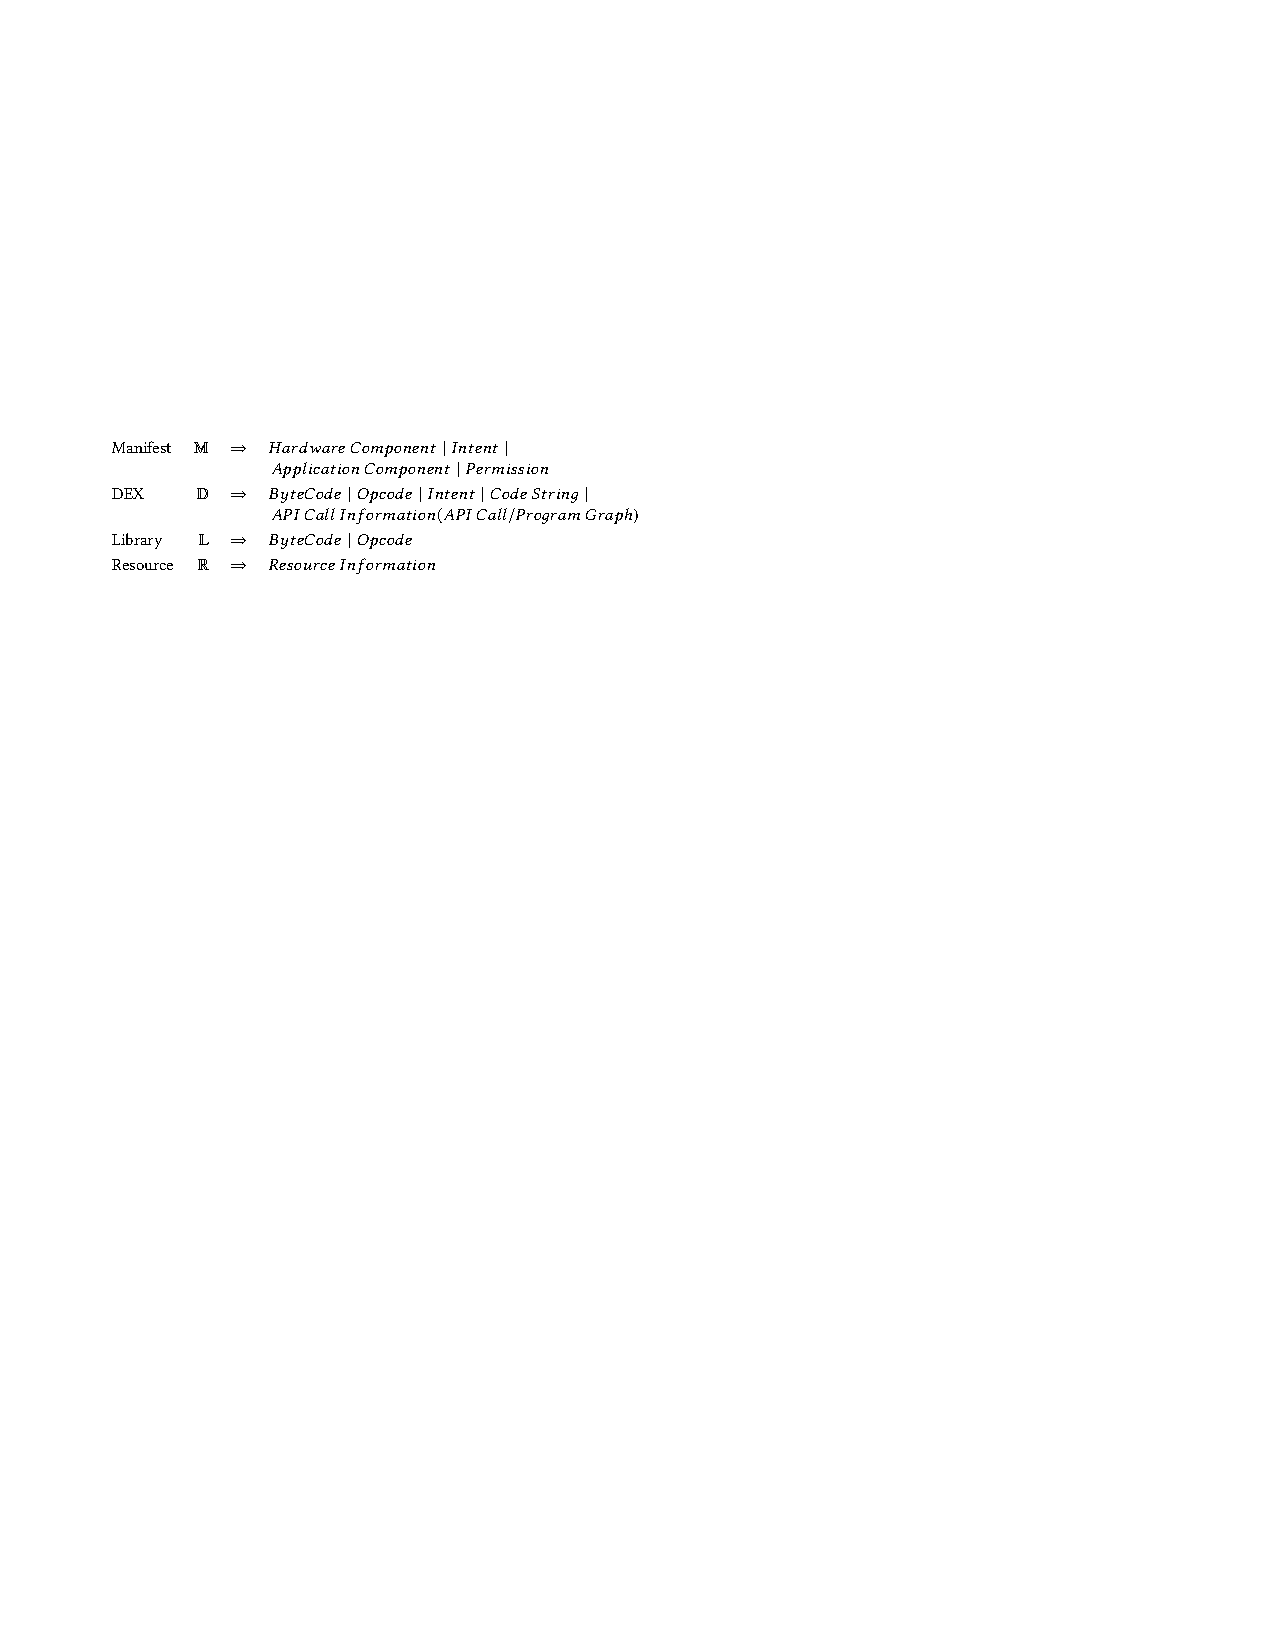
\includegraphics[width=0.68\linewidth]{fig/features.pdf}
    \vspace{-0.2cm}
    \caption{APK files and their corresponding features.}
    \label{fig:features}
    \vspace{-0.6cm}
\end{figure}

\featurepoint{[M|D]}{Intent}
As the primary ways of communication among components, intents connect various Application Components and delineate standard operations one app can perform.
% As the primary ways of communication among components, intents take responsibility for initiating Activities, managing Services lifecycle, and delivering information to Broadcast Receivers.
They are pivotal in initiating Activities, managing Services lifecycle, and delivering broadcast information to Broadcast Receivers.
Malware often monitors these communication status to trigger malicious actions, such as activating pre-configured malicious activities~\cite{zhou2012hey}.
Approaches~\cite{li2021robust,feng2020performance,xu2016iccdetector} aim to capture these malicious behaviors by analyzing corresponding intents.


% Towards this end, intents have been extensively employed to capture potential malicious activities~\cite{feng2020performance,li2021robust,xu2016iccdetector}.

% Approaches like MobiTive~\cite{feng2020performance} and RAMDA~\cite{li2021robust} utilize intents specified in the manifest for malware detection.
% Meanwhile, ICCDetector~\cite{xu2016iccdetector} integrates intents from the manifest and the application's codebase to model the application's behaviors.

\featurepoint{[M]}{Permission}
Android employs a permission-based mechanism to regulate access to sensitive data and restricted actions.
For an app to carry out particular actions, it must obtain the requisite permissions~\cite{au2012pscout,backes2016demystifying}.
The set of permissions required by an app can thus offer insights into its intended behaviors.
Particularly, malware often demands permissions that are unnecessary for benign apps to execute malicious actions~\cite{enck2009lightweight}.
Consequently, numerous Android malware detectors~\cite{he2022msdroid,xu2018deeprefiner,arp2014drebin,kim2018multimodal,wu2021android} capture the differences to distinguish malware. 


% Consequently, numerous malware detection frameworks~\cite{arp2014drebin,xu2018deeprefiner,kim2018multimodal,wu2021android,he2022msdroid} employ permissions as a key heuristic in distinguishing malware.


\featurepoint{[D]}{API Call Information (API Call and Program Graph)}
% \jiahao{Merge API call with its connections}
% \jh{API Call Information is a widely used feature source in Android malware detection, consisting of API calls and their connections.
% Android apps make use of API calls to tap into the operating system's functionality and system resources~\cite{peiravian2013machine}.
% For instance, calling the \textit{sendTextMessage()} indicates that the app is likely to send a text message.
% Additionally, the API calls are often connected with each other to form a program graph, where each node signifies a method, and each edge denotes a method invocation~\cite{li2023black}, illustrating the app's structural information~\cite{wu2019malscan}.}
% \red{For clarity, we decouple API Call Information into two sub-categories: \textit{API Call} refers to the API calls themselves, while \textit{Program Graph} denotes the connections between API calls.}
API Call Information, consisting of API calls and their connections, is a widely utilized feature source in Android malware detection.
Android apps make use of these API calls to access the operating system's functionality and system resources~\cite{peiravian2013machine}.
For instance, the invocation of \textit{sendTextMessage()} suggests that the app is likely to send a text message.
Furthermore, API calls are connected to form a graph, where each node signifies a method, and each edge denotes a method invocation~\cite{li2023black}, illustrating the app's structural information~\cite{wu2019malscan}.
For clarity, we differentiate API Call Information into two sub-categories: \textit{API Call}, referring to the individual API calls, and \textit{Program Graph}, denoting the relationships among these API calls.
Numerous studies~\cite{arp2014drebin,kim2018multimodal,wu2021android} detect sensitive API calls (\textit{e.g., getDeviceId()}) to estimate the probability of an app being malicious.
In contrast, other solutions~\cite{wu2019malscan,he2022msdroid,hou2017hindroid,xu2020sdac,martin2017evolving,ye2019out} venture deeper, examining the relationships between API calls to capture an app's semantics for malware detection.

\featurepoint{[D|L]}{ByteCode and Opcode}
Similar to previous research~\cite{xu2018deeprefiner,sun2016taintart,li2021palmtree,daoudi2021dexray}, we treat both the \textit{raw bytecode} and the \textit{assembly code} derived from the \textit{Dex} and \textit{Library} as ByteCode.
ByteCode contains a sequence of instructions, where each instruction consists of a single Opcode and several operands.
The Opcode denotes a specific operation; for instance, the \texttt{invoke} means a method invocation.
The operands provide additional information for the Opcode, such as the method name.
In addition, ByteCode and Opcode from the \textit{Dex} and \textit{Library} offer insights into the static execution flows of apps' Java and Native codes, providing a view of how an app work~\cite{kim2018multimodal}.
Recent research attempts to represent Bytecode and Opcode in various formats, such as image~\cite{mclaughlin2017deep,hsien2018r2,amin2022android,xiao2019image} and text~\cite{xu2018deeprefiner,yan2018lstm,karbab2021petadroid}, to capture apps' semantics.

% Consistent with previous studies~\cite{xu2018deeprefiner,sun2016taintart,li2021palmtree}, we consider the assembly code derived from the decompilation of DEX and Library files as another kind of bytecode representation of an application.
% Both bytecode and opcode preserve the original characteristics of an application, providing a holistic perspective on the programming behaviors the application executes.

\featurepoint{[D]}{Code String}
Apps often embed key information like URLs and IP addresses as string values within their codebase.
These strings can be traced in the assembly code, tagged either as \texttt{const-string} or \texttt{const-string/jumbo}. 
Such strings can provide crucial clues about potential malicious activities~\cite{arp2014drebin}.
For instance, malware sets up network sockets to communicate with remote servers, using the string \texttt{socket} in the codebase.
A number of works~\cite{arp2014drebin,kim2018multimodal,zhu2019transparent} have used code strings to identify potential illegal operations.

% With the evidence provided by research like~\cite{arp2014drebin,kim2018multimodal,zhu2019transparent}, it is clear that code string has become a significant feature in malware detection.

% Therefore, it is unsurprising that it has been widely adopted as a feature source in Android malware detection~\cite{arp2014drebin,kim2018multimodal,zhu2019transparent}.
% Accordingly, some approaches~\cite{arp2014drebin,kim2018multimodal,zhu2019transparent} have tapped into these strings as indicators for malware detection.

% \featurepoint{[D]}{Program Graph}
% The program graph encapsulates the caller-callee relationships among the methods inside an app as a directed graph, where each node signifies a method, and each edge denotes a method invocation~\cite{li2023black}.
% \jh{In essence, the program graph illustrates the app's structural information, 
% offering a holistic perspective on the app's behavior~\cite{wu2019malscan}.}
% When leveraging program graphs for malware detection, a prevalent strategy is to re-envision them as other constructs (\textit{e.g.}, as a social network) and subsequently employ corresponding techniques to extract valuable insights~\cite{wu2019malscan,wu2021homdroid}.
% Alternatively, some researchers directly apply powerful techniques, like graph neural network (GNN), to distill pertinent information from the program graph itself~\cite{mariconti2016mamadroid,he2022msdroid,gao2021gdroid}.

% To distill helpful information for malware detection, one popular selection is treating the program graph as a social network and apply related techniques to extract information~\cite{wu2019malscan,wu2021homdroid}.
% Another direction is to simplify the graph structure to capture meaningful information~\cite{mariconti2016mamadroid,he2022msdroid}.
% To utilize this information, one direction~\cite{wu2019malscan,wu2021homdroid} treats the program graph as a social network and performs centrality and homophily analysis~\cite{dehghani2016purity,fiore2005homophily}.
% Another direction is to simplify the graph structure to capture meaningful information~\cite{mariconti2016mamadroid,he2022msdroid}.
% There are also some approaches~\cite{} directly extract information from the program graph to detect malware.

% To preserve the program semantic information, MalScan~\cite{wu2019malscan} and HomDroid~\cite{wu2021homdroid} treat the program graph as a social network and perform centrality and homophily analysis~\cite{dehghani2016purity,fiore2005homophily}.

% Also, some approaches have attempted to simplify the graph structure to capture meaningful information. 
% For example, MamaDroid~\cite{mariconti2016mamadroid} abstracts the graph based on family and package details.
% MsDroid~\cite{he2022msdroid} derives subgraphs rooted with sensitive API calls to describe potential malicious operations.

\featurepoint{[R]}{Resource Information}
Apps utilize resources to house traditional files and static elements, such as bitmaps and animation instructions.
These resources are generally decoupled from the application codebase for ease of maintenance.
Attackers sometimes embed malicious code within resource files, like image files, as a tactic to evade detection.
Approaches like DeepRefiner~\cite{xu2018deeprefiner} consider resource information as a crucial feature source for malware detection.
% This stems from the fact that resources typically house traditional and static elements, such as bitmaps and animation instructions. 
% Attackers sometimes embed malicious code within resource files, like image files, as a tactic to evade detection.

% Resources refer to the traditional files and static elements leveraged by your application, such as bitmaps, layout definitions and animation instructions.
% These resources are generally decoupled from the application codebase for ease of maintenance. 
% During runtime, Android selects the most suitable resource based on the device's current configuration
% In some instances, attackers may insert malicious code into resource files, such as image files, as a tactic to elude detection.

% \featurepoint{[DY]}{Dynamic features}
% \jh{dynamic features are collected during runtime, and they are not included in the APK file. For example, the network traffic, the system traces, and the system calls. These information can reflected the app's runtime behaviors. It is time consuming to collect these features.}

\begin{figure}[t]
    \centering
    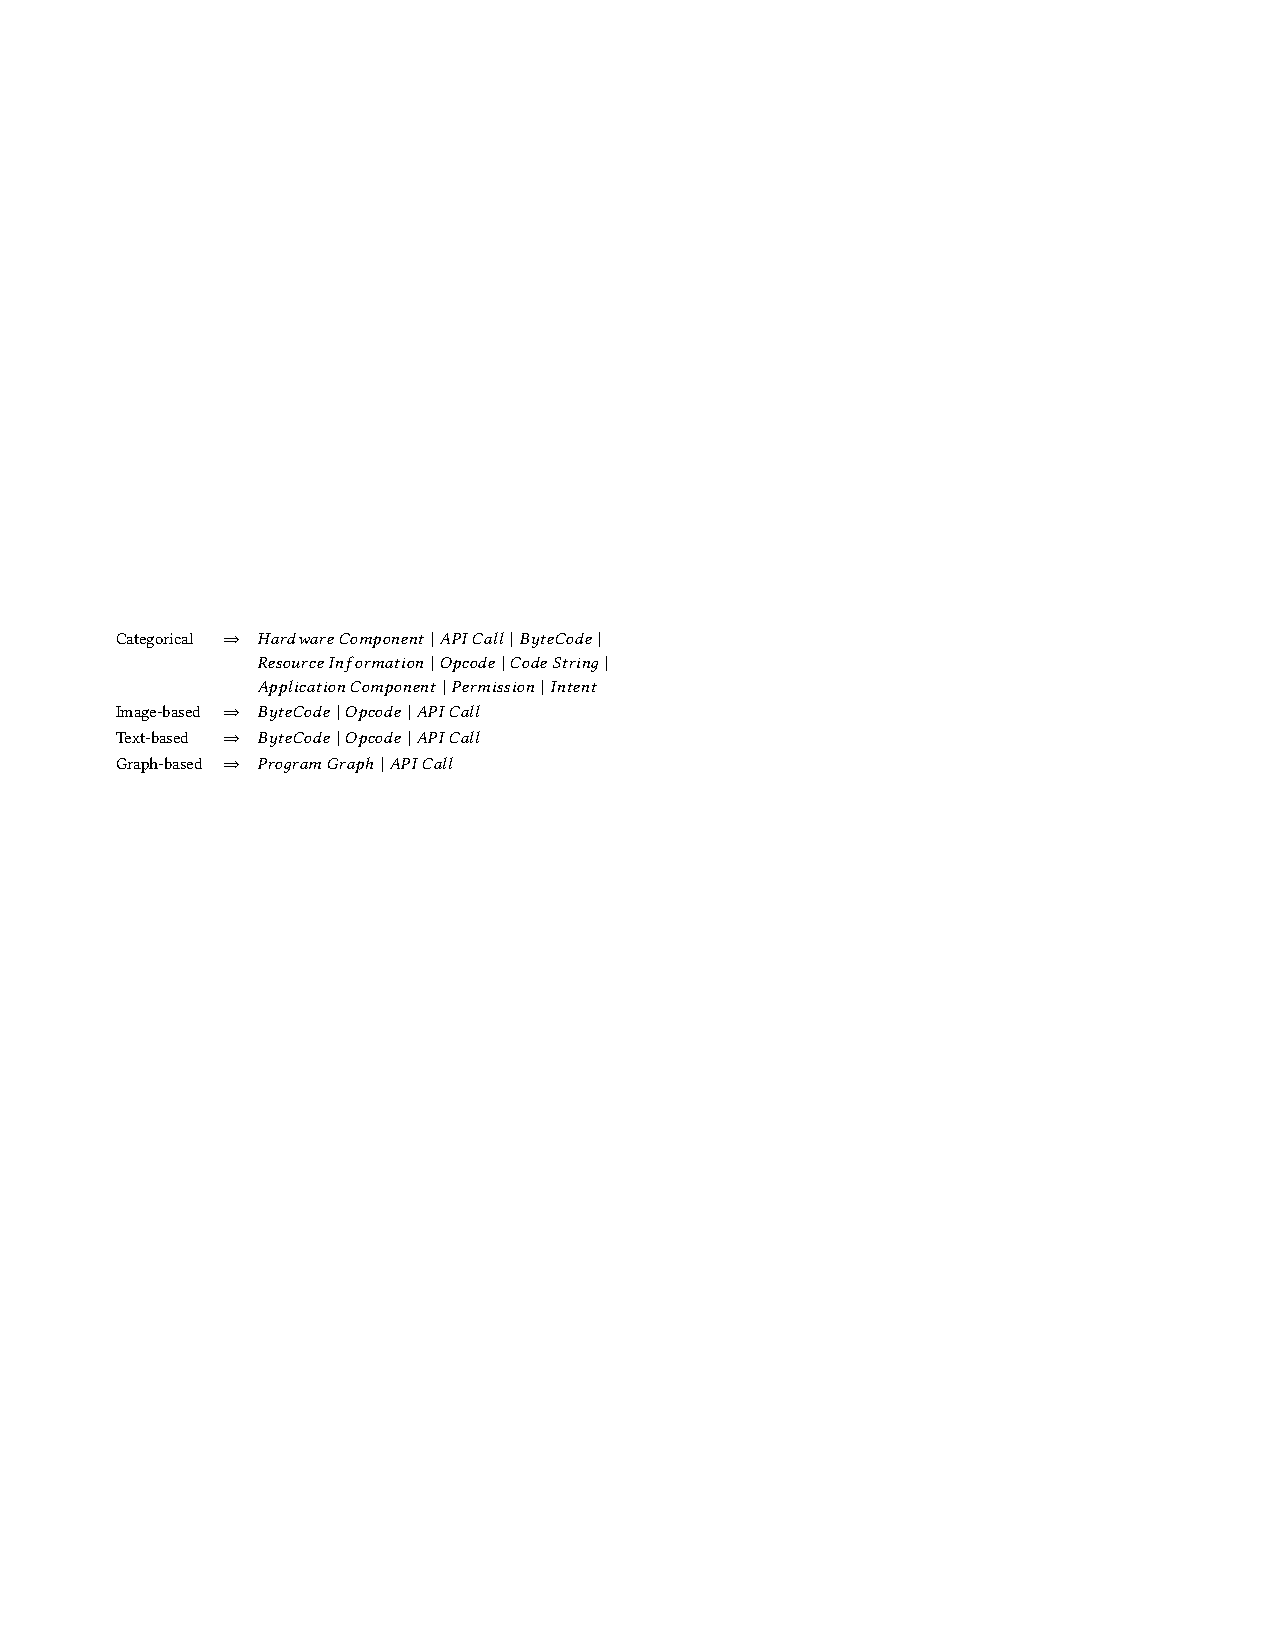
\includegraphics[width=0.68\linewidth]{fig/representation.pdf}
    \vspace{-0.1cm}
    \caption{The relationships between Feature Representations and widely used APK Features.}
    \label{fig:representation}
    \vspace{-0.5cm}
\end{figure}

\subsection{Feature Representation}
\label{sub:apk_feature_encoding}
APK characterizations provide multi-perspective views of an app's behavior.
Before these features can be fed into ML models, they must be encoded into representations that the models can interpret.
Broadly, the encoding process falls into four categories: categorical, image-based, text-based, and graph-based.
\jh{Figure~\ref{fig:representation} illustrates the relationships between these encoding strategies and the corresponding APK features.}
In the following section, we discuss each encoding strategy in detail.

% Some approaches~\cite{yuan2014droid,arp2014drebin,li2019adversarial,feng2019mobidroid,li2021robust,wu2021android,hou2017hindroid} encode these features into a binary vector, where each position indicates whether a specific feature exists or not.
% Alternatively, another approach showcased in~\cite{kim2018multimodal} calculates the frequency of each feature to obtain a vector of real numbers.
\bulletpoint{Categorical encoding}
Features like hardware components, intents, and code strings are often viewed as categorical data and can be easily transformed into numerical values.
A widely-encoding strategy is to convert these features into a binary vector, where each position indicates whether a specific feature exists or not~\cite{arp2014drebin,hou2017hindroid,li2021robust,wu2021android,yuan2014droid,li2019adversarial,feng2019mobidroid}.
On the other hand, another line of research~\cite{kim2018multimodal} calculates the frequency of each feature to obtain a vector of numerical values, reflecting the importance of each feature.

\bulletpoint{Image-based encoding}
% Note: the bytecode definition
% Several approaches~\cite{daoudi2021dexray,ding2020android,mclaughlin2017deep,hsien2018r2,zegzhda2018applying,he2019malware,xiao2019image,yuan2020byte} depict bytecode or opcode sequences in the form of images, subsequently feeding them into a convolutional neural network (CNN) to extract features. 
% In Android malware detection, it is a prevalent practice to represent bytecode or opcode sequences as images.
% Various solutions~\cite{daoudi2021dexray,ding2020android,hsien2018r2,xiao2019image,mclaughlin2017deep} visualize the bytecode or opcode sequences as image forms, subsequently extracting information from these depictions.
% Notably, \textsc{DexRay}~\cite{daoudi2021dexray} transforms the app's bytecode into grey-scale vector images, wherein each pixel corresponds to a distinct byte.
% Additionally, some approaches map various features to images to represent the APK. 
% For instance, Zegzhda et al.~\cite{zegzhda2018applying} attempt to map the sequence of API calls combined with protection levels to an RGB image.
Representing specific features as images and leveraging image processing techniques is a well-established approach in malware detection.
Specifically, bytecode and opcode are often visualized as images to describe apps' behaviors~\cite{mclaughlin2017deep,daoudi2021dexray,hsien2018r2,xiao2019image,ding2020android}.
Notably, \textsc{DexRay}~\cite{daoudi2021dexray} transforms the app's bytecode into grey-scale vector images, wherein each pixel corresponds to a distinct byte.
In a similar vein, some other features are also mapped to images to depict the APK's characteristics.
For instance, Zegzhda et al.~\cite{zegzhda2018applying} combine API calls with protection levels as an RGB image.

\bulletpoint{Text-based encoding}
% Bytecode and opcode sequences can be analogized to textual data.
% Many existing approaches~\cite{xu2018deeprefiner,karbab2018maldozer,karbab2021petadroid,xu2020sdac,sun2019scalable} regard apk characterization as textual data and leverage natural language processing (NLP) techniques to enhance android malware detection.
% By considering API calls as \texttt{words} and their sequences as \texttt{sentences}, methods presented in~\cite{karbab2018maldozer,karbab2021petadroid,xu2020sdac} utilize word embedding techniques, such as Word2Vec~\cite{mikolov2013distributed}, to extract semantic information included in the API calls.
% Separately, Sun et al.~\cite{sun2019scalable} treat API calls and permissions as sparse data, applying Doc2Vec~\cite{le2014distributed} to derive their vector representations.
Text-based encoding is also a widely used strategy in Android malware detection.
Many existing methods~\cite{xu2018deeprefiner,xu2020sdac,karbab2021petadroid,karbab2018maldozer,sun2019scalable} have approached APK features from a textual perspective, employing natural language processing (NLP) techniques to amplify detection capability.
For example, by considering API calls as \texttt{words} and their sequences as \texttt{sentences}, methods presented in~\cite{xu2020sdac,karbab2021petadroid,karbab2018maldozer} utilize word embedding techniques, such as Word2Vec~\cite{mikolov2013distributed}, to extract semantic information included in the API calls.
Separately, Sun et al.~\cite{sun2019scalable} treat API calls and permissions as sparse data, applying Doc2Vec~\cite{le2014distributed} to derive their vector representations.

\bulletpoint{Graph-based encoding}
Recently, graph structure has been widely adopted to represent apps' semantics~\cite{he2022msdroid,li2023black}.
One direction is to leverage program graphs to model APK behaviors~\cite{wu2019malscan,wu2021homdroid,he2022msdroid,pektacs2020deep,pektacs2020learning}.
Another avenue aims to build API-based feature graphs, drawing insights from API calls and their meta-relationships. 
An example is to identify whether two API calls are in the same block, thereby capturing the app's intended operations~\cite{hou2017hindroid,huang2019deep}.
When these features are represented as graphs, graph-based techniques (\textit{e.g.,} Graph2Vec~\cite{narayanan2017graph2vec}, social network~\cite{wu2019malscan}) are employed to extract apps' structural information.



% \vspace{-0.1cm}
\subsection{Machine Learning Modeling}
\label{sub:ml_models}
% Subsequent to encoding, learning models are leveraged to identify underlying patterns from the encoded features, facilitating informed predictions.
After encoding these features as numerical vectors, machine learning models are leveraged to identify malicious patterns.
Following previous studies~\cite{qiu2020survey,zhao2021impact}, we categorize the models employed in Android malware detection into two main categories: traditional machine learning (TML) and deep learning (DL) models.
TML models, such as linear regression or decision trees, typically exhibit simpler structures that can explicitly model the relationship between input and output. 
As such, these TML models often require domain knowledge to extract features from input data.
In contrast, DL models are characterized by their multiple layers of neurons, enabling them to capture complex non-linear mappings from input to output~\cite{zhao2018deepsim}.
This capability means that DL models are less reliant on domain knowledge during the feature extraction.
In this section, we provide a concise introduction to the widely used models.
%  in Android malware detection.

\bulletpoint{TML models}
% SVM~\cite{arp2014drebin,hou2017hindroid,xu2020sdac,sun2016sigpid,garcia2018lightweight}
% KNN~\cite{wu2019malscan,wu2021homdroid,wu2016effective,aafer2013droidapiminer}
% RF~\cite{mariconti2016mamadroid,zhu2018hemd}
% DT~\cite{zarni2013permission,yerima2014android}
% (SVM)~\cite{noble2006support}
% (KNN)~\cite{peterson2009k} (RF)~\cite{breiman2001random}
Given APK features, TML models are commonly employed to discern patterns from them.
The Support Vector Machine (SVM) can find one hyperplane that separates the high-dimensional data points with varying labels.
This capability has made it a popular choice to detect Android malware~\cite{arp2014drebin,hou2017hindroid,xu2020sdac,sun2016sigpid,garcia2018lightweight}.
K-Nearest Neighbors (KNN) has also been applied in Android malware detection~\cite{wu2019malscan,wu2021homdroid,aafer2013droidapiminer,wu2016effective}.
This algorithm identifies the nearest neighbors of a given sample and subsequently classifies the sample based on the majority label of its neighbors.
Additionally, as an ensemble-based learning method, Random Forest (RF) creates a forest of decision trees, each trained on a random subset of the data.
This approach capitalizes on the strength of multiple decision trees, making the model more robust and accurate than individual trees.
Such advantages have led to its significant application in malware detectors~\cite{mariconti2016mamadroid,zhu2018hemd}.

\bulletpoint{DL models}
DL models have exhibited strong capability in modeling malware behaviors. 
This part provides an insight into the widely used DL models tailored for Android malware detection.
% Multi-Layer Perceptron (MLP) is a fundamental model composed of multiple layers of neurons and has been applied in various studies~\cite{kim2018multimodal,li2021robust,martin2017evolving,sun2019scalable,zhu2019fsnet,chen2020denas}.
As a basic feed-forward neural network, Multi-Layer Perceptron (MLP), composed of several layers of neurons, \jh{has shown significant effectiveness in detecting Android malware~\cite{kim2018multimodal,li2021robust,martin2017evolving,sun2019scalable,zhu2019fsnet,chen2020denas}.}
The Recurrent Neural Network (RNN)~\cite{medsker2001recurrent} is a type of neural architecture that can capture the sequential information of input data.
By representing APK features (\textit{e.g.}, API calls and bytecode) as sequences, existing solutions~\cite{xu2018deeprefiner,yan2018lstm,vinayakumar2017deep} leverage RNN to explore the temporal dependencies embedded in these features.
The Convolutional Neural Network (CNN)~\cite{he2017mask} is equipped with multiple convolutional and pooling layers, enabling it to recognize contextual information derived from low-level features~\cite{girshick2015fast}.
This intrinsic capability makes it especially effective in capturing patterns from image-oriented data.
Reflecting its efficacy, CNN has been extensively employed to extract malicious patterns from image-based features in Android malware detection~\cite{mclaughlin2017deep,hsien2018r2,feng2019mobidroid,karbab2018maldozer,huang2019deep,he2019malware}.
Given the graph representation of APK features (\textit{e.g.,} program graphs), Graph Neural Network (GNN)~\cite{kipf2016semi} can facilitate malware detection~\cite{he2022msdroid,mariconti2016mamadroid,gao2021gdroid,fan2021heterogeneous}.
This is because GNN can effectively propagate and aggregate node information along graph edges, thereby capturing the structural information of apps.
% some approaches~\cite{he2022msdroid,gao2021gdroid,fan2021heterogeneous} have attempted to tailor Graph Neural Networks (GNN) to facilitate malware detection.
Utilizing a process of encoding and subsequently decoding input features, Autoencoders (AE) have the capacity to generate refined data representations, which makes it a popular choice in detecting malware~\cite{li2021robust,yang2021cade,zhu2021hybrid}.

In addition, existing research~\cite{su2016deep,wang2020sedroid,amin2022android} also tries to explore the potential of other DL models, like generative adversarial network (GAN)~\cite{goodfellow2014generative} and deep belief network (DBN)~\cite{hinton2009deep}.
For instance, Amin et al.~\cite{amin2022android} employ the dual-network structure of GAN --- one generates malware samples and the other works to distinguish these samples --- to enhance the malware detection capability.


% \begin{center}
%     \begin{conclusionbox}
%     \textit{Finding:} 
%     \jh{Central to static and ML-based Android malware detection is how to effectively \textit{profile apps' behaviors} and how to \textit{leverage suitable ML models} to unveil malicious patterns.}
%     \end{conclusionbox}
% \end{center}

\begin{center}
    \begin{conclusionbox}
    \textit{Finding:} 
    \jh{At the core of static and ML-based Android malware detection lies the ability to accurately \textit{profile app behaviors} and to \textit{select and leverage appropriate ML models} that can effectively uncover malicious patterns. Achieving this requires not only expressive feature representations but also a careful alignment between behavioral semantics and model capabilities.}
    \end{conclusionbox}
\end{center}

% \subsection{Summary}
% \label{sub:summary}
% Quick summarize this section, and use some motivation to illustrate we need to conduct a quantitative analysis on the primary techniques.


% \begin{table*}[t]
% \centering
% \caption{
% % (\textit{AndroidManifest.xml} for Manifest, \textit{classes*.dex} for Dex, \textit{res/*} for Resource, and \textit{*.so} for Library)
% An overview of the 12 representative approaches we selected from major venues in security, software engineering, and machine learning. 
% \ymark \ indicates that the APK file (e.g., \textit{AndroidManifest.xml} for Manifest) is taken as input in Android malware detection, while \nmark \ is the opposite.
% \cmark \ and \xmark \ indicate whether feature engineering is handcrafted using domain knowledge or learned using representation learning.
% The effectiveness we present is based on the results reported in the original papers.}
% \begin{adjustbox}{width=0.85\linewidth}
% \begin{tabular}{@{}c|cc|cccc|cc|rr|rrr@{}}
% \toprule
% \multirow{2}{*}{\raisebox{-0.3cm}{\textbf{\begin{tabular}[c]{@{}c@{}}Selected \\ Approach\end{tabular}}}} & \multicolumn{2}{c|}{\textbf{Publication}} & \multicolumn{4}{c|}{\textbf{Input from APK}} & \multicolumn{2}{c|}{\textbf{Feature Engineering}} & \multicolumn{2}{c|}{\textbf{Dataset}} & \multicolumn{3}{c}{\textbf{Effectiveness}} \\ \cmidrule(lr){2-3} \cmidrule(lr){4-7} \cmidrule(lr){8-9} \cmidrule(lr){10-11} \cmidrule(l){12-14}
%  & \textbf{Venue} & \textbf{Year} & \textbf{Manifest} & \textbf{Dex} & \textbf{Resource} & \textbf{Library} & \textbf{Handcrafted} & \textbf{Learned} & \textbf{Malware} & \textbf{Goodware} & \textbf{TPR} & \textbf{FPR} & \textbf{F1} \\ \midrule
% Drebin\cite{arp2014drebin} & NDSS & 2014 & \ymark & \ymark & \nmark & \nmark & \cmark & \xmark & 5,560 & 123,453 & 94\% & \textbf{1\%} & 87\% \\ \midrule
% % ICCDetector\cite{xu2016iccdetector} & TIFS & 2016 & \ymark & \ymark & \nmark & \nmark & & & 5,264 & 12,026 & 93\% & \textbf{1\%} & 96\% \\ \midrule
% MamaDroid\cite{mariconti2016mamadroid} & NDSS & 2017 & \nmark & \ymark & \nmark & \nmark & \cmark & \xmark & 35,493 & 8,447 & 97\% & 2\% & 96\% \\ \midrule
% Mclaughlin et al.\cite{mclaughlin2017deep} & CODASPY & 2017 & \nmark & \ymark & \nmark & \nmark & \xmark& \cmark & 13,637 & 13,758 & 95\% & \textbf{1\%} & 97\% \\ \midrule
% HinDroid\cite{hou2017hindroid} & KDD & 2017 & \nmark & \ymark & \nmark & \nmark & \cmark & \xmark & 1,216 & 1,118 & \textbf{99\%} & 2\% & \textbf{99\%} \\ \midrule
% DeepRefiner\cite{xu2018deeprefiner} & EuroS\&P & 2018 & \ymark & \ymark & \ymark & \nmark & \xmark & \cmark & 62,915 & 47,525 & 98\% & 2\% & 98\% \\ \midrule
% Kim et al.\cite{kim2018multimodal} & TIFS & 2018 & \ymark & \ymark & \nmark & \ymark & \cmark & \cmark & 21,260 & 20,000 & \textbf{99\%} & \textbf{1\%} & \textbf{99\%} \\ \midrule
% MalScan\cite{wu2019malscan} & ASE & 2019 & \nmark & \ymark & \nmark & \nmark & \cmark & \xmark & 15,430 & 15,285 & --- & --- & 98\% \\ \midrule
% SDAC\cite{xu2020sdac} & TDSC & 2020 & \nmark & \ymark & \nmark & \nmark & \xmark & \cmark & 34,497 & 35,645 & 98\% & \textbf{1\%} & \textbf{99\%}\\ \midrule
% HomDroid\cite{wu2021homdroid} & ISSTA & 2021 & \nmark & \ymark & \nmark & \nmark & \cmark & \xmark & 3,358 & 4,840 & 97\% & 4\% & 95\% \\ \midrule
% Xmal\cite{wu2021android} & TOSEM & 2021 & \ymark & \ymark & \nmark & \nmark & \cmark & \xmark & 15,570 & 20,120 & 98\% & 2\% & 98\% \\ \midrule
% RAMDA\cite{li2021robust} & WWW & 2021 & \ymark & \ymark & \nmark & \nmark & \cmark & \xmark & 21,621 & 36,862 & 93\% & \textbf{1\%} & 90\% \\ \midrule
% MSDroid\cite{he2022msdroid} & TDSC & 2022 & \nmark & \ymark & \nmark & \nmark & \cmark & \xmark & 30,210 & 51,580 & 97\% & \textbf{1\%} & 97\% \\ \bottomrule
% \end{tabular}
% \end{adjustbox}
% \centering
% \begin{tablenotes}
% \footnotesize
% \item \ \ TPR, FPR, and F1 refer to true positive rate, false positive rate, and F1-score. 
% As MalScan is only evaluated on F1, its TPR and FPR are not available.
% \end{tablenotes}
% \label{tab:literature}
% \vspace{-0.4cm}
% \end{table*}
